\documentclass[a4paper, 12 pt]{article}

\usepackage{multicol}
\usepackage{hyperref}
\usepackage{graphicx}
\graphicspath{ {images/} }

\begin{document}

\title{
  Crivo de Eratóstenes Paralelo usando MPI \\
  \large Relatório da Programação Paralela da Universidade Federal do ABC}
\author{Hiago Lucas Cardeal de Melo Silva - 11077315}
\date{\today}
\maketitle

\section{Metodologia}

O método utilizado aqui tem como ideia base aproveitar o máximo do cache dos processadores. Portanto,
o objetivo central é evitar \textit{cache-miss}. Para isso, utilizou-se uma implementação pouco intuitiva, 
onde o \textit{array} de $n$ números é dividido para os $p$ processos e, cada $subarray$ restante é novamente dividido dentro de cada processo
de forma que cada partiçao ocupe o máximo de \textit{cache} possível.

\begin{enumerate}

\item A primeira etapa de cada processo é calcular a porção de números que deverá ser processado por ele. Uma das otimizaçoes
feitas aqui é considerar apenas números ímpares.

\item Após a divisao de todos os números que serão calculados pelo processo atual, este novo
\textit{array} de números é novamente dividido igualmente em outros $cache\_length$ \textit{arrays}. Onde $cache\_length$ é
o número de linhas de cache somando-se os caches L1, L2 e L3. O número $cache\_length$ é obtido através da função
\textit{get\_best\_cache\_length}. Suponha como sendo $C$ o conjunto dos $cache\_length$ \textit{arrays} restantes.

\item Calcula-se então, de forma sequencial, os números primos entre $0$ e $\sqrt(n)$. Suponha que $P$ representa
o conjunto de números primos entre $0$ e $\sqrt(n)$.

\item Este é o principal passo do algoritmo. Se trata da organização de dois \textit{loops}. O primeiro \textit{loop} itera
para cada \textit{subarray} em $C$, armazenando este \textit{subarray} no cache. O segundo loop itera por todos os números primos. Estes também sao armazenados no cache.
Com esta estrutura, o número de $cache-miss$ é diminuido drásticamente. O pseudocódigo desta estapa pode ser encontrada na figura \ref{fig:pseudo}.

\item Finalmente, realiza-se um \textit{Reduce} para somar a quantidade de primos em cada processo.

Note que inicialmente, cada processo realiza exatamente os mesmos procedimento dos demais. Apenas na ultima etapa é que ocorre uma comunicação
para somar os primos encontrados. Sendo assim, a \textbf{distribuição de carga} entre os processadores é praticamente a mesma.

\begin{figure}[h]
    \centering
    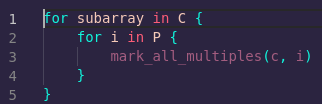
\includegraphics[width=0.6\textwidth]{figure-0.png}
    \caption{Pseudo código da etapa 4.}
    \label{fig:pseudo}
\end{figure}

\end{enumerate}

\section{\textit{Speedup} e Eficiencia}

A máquina utilizada para os testes possui as seguintes especificações:

\begin{itemize}
  \item 8 GB de RAM
  \item Processador Intel(R) Core(TM) i5-8250U CPU @ 1.60GHz
  \item 4 \textit{cores}
  \item 2 \textit{threads} por \textit{core}
  \item 32K de cache L1d / L1i
  \item 256K de cache L2
  \item 6144K de cache L3
\end{itemize}

Como base para o algorítmo sequencial foi utilizado o crivo implementado em Stack Exchange
\href{ https://codereview.stackexchange.com/questions/112901/eratosthenes-sieve-optimized-in-c}{(link)}
como resposta à um \textit{code review}. Esta implementaçao foi uma das mais eficientes encontradas, e, 
portanto, a análise dos \textit{speedups} terá melhor precisão.

A algorítmo sequencial utilizado nao possui boa escalabilidade de memória, portanto, nao foi possível usa-lo para
valores maiores que $2 * 10^{10}$

\begin{figure}[h]
  \centering
  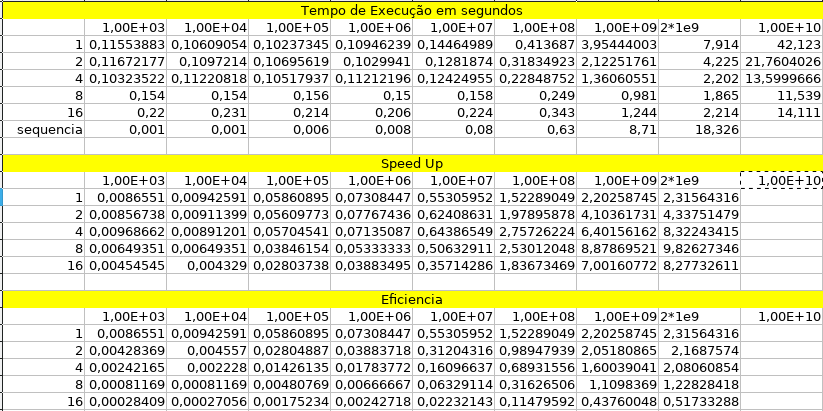
\includegraphics[width=0.8\textwidth]{figure-1.png}
  \caption{Tabela de resultados para tempo de execução, speedup e eficiencia.}
  \label{fig:table}
\end{figure}

\begin{figure}[h]
    \centering
    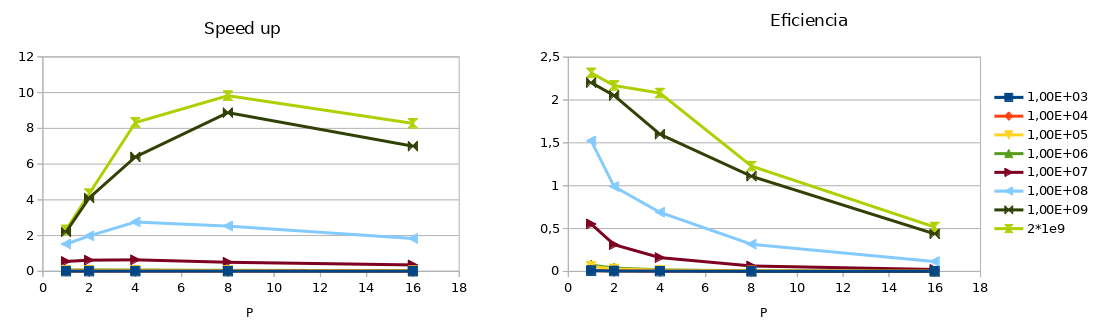
\includegraphics[width=1\textwidth]{figure-2.png}
    \caption{Speedup e eficiência.}
    \label{fig:speedups}
\end{figure}

\subsection{Análise do \textit{speedup}}
A implementaçao paralela feita aqui calcula parte dos primos (de $0$ até $\sqrt{n}$) de forma sequencial.
Apenas a outra porção ($\sqrt{n}$ até $n$) é calculada paralelamente. Se $n$ for pequeno uma grande porção
dos números será processdo sequencialmente, o que diminui a eficiência do algoritmo.

Além disso, com uma entrada pequena de dados, os \textit{caches} dos processadores podem não ser totalmente aproveitados.

É possível notar na figura \ref{fig:speedups} que até $10^7$ a implementação apresenta \textit{speedups} menores que $1$ e, portanto, 
a utilizaçao deste método nao é justificável. No entanto para valores mais altos de o \textit{speedup} aumenta drásticamente.
\\\\
Uma outra análise que pode ser feita sobre os \textit{speedups} é referente ao seu comportamento
à partir de 4 processadores. 

A máquina onde os testes foram feitos possui $4$ \textit{cores}, contendo cada um $2$ \textit{threads}.
Embora existam apenas $4$ \textit{cores} disponíveis, o pico de \textit{speedup}
se encontra no $8$. Isto ocorre pois o sistema operacional é capaz de alternar entre as 2 \textit{threads} 
durante os períodos de \textit{stall}.
\\\\
A partir de $16$ processos o \textit{speedup} começa a cair, pois o número de \textit{cores} 
é ultrapassado e apenas o custo de \textit{overhead} aumenta.

\subsection{Eficiencia e escalabilidade}

Como é possível observar na figura \ref{fig:speedups}, o aumento do número de processos
faz com que a eficiencia do algoritmo caia. Isto ocorre pois os \textit{caches} dos
processadores são menos aproveitados uma vez que os dados estao mais dividídos. Portanto, para aumentar a
eficiência deve-se aumentar a entrada.

Este comportamento caracteriza um algoritmo com \textbf{escalabilidade fraca}.

\section{Resultados}

\subsection{Quantidade de primos entre 0 e 1.000.000.000}
50847534

\subsection{Lista dos 20 ultimos primos entre 0 e 1.000.000.000}

Em ordem decrescente.

\begin{multicols}{4}
  \begin{enumerate}
    \item 999999937
    \item 999999929
    \item 999999893
    \item 999999883
    \item 999999797
    \item 999999761
    \item 999999757
    \item 999999751
    \item 999999739
    \item 999999733
    \item 999999677
    \item 999999667
    \item 999999613
    \item 999999607
    \item 999999599
    \item 999999587
    \item 999999541
    \item 999999527
    \item 999999503
    \item 999999491
  \end{enumerate}
\end{multicols}

\end{document}